\chapter{Multiple Integrated Applications (MIA)}
\pagestyle{fancy}

MIA is designed to be a collection of scripts, tools, programs, and commands that have been created in the past and may be useful in the future. It's original idea was a place for the original author to combine all of his previous applications and codes into one location that can be compiled cross platform. MIA is written in C++ but will contain codes that were originally designed in C\#, Java, Python, and others. MIA is created for the authors personal use but may be used by others if a need or desire arises under the terms of Antonius’ General Purpose License (AGPL). 

The MIA acronym was created by the original author for the sole purpose of this application. The design of MIA is a terminal prompt that accepts commands. There are no plans to convert MIA into a GUI application as there is currently no need; however, some elements may be programmed in that produce a GUI window for certain uses such as graphs. The MIA manual is designed to be an explanation of what MIA contains as well as a guide of how to utilize the MIA program to it's fullest. 

As MIA is continually under development, this document is also. Due to this, it may fall behind and become slightly outdated as I implement and test new features into MIA. I will attempt to keep this document up to date with all of the features MIA contains but I can only do so if time permits.

\section{Setting up the MIA Environment for Developers - Linux}

To set up MIA for development, simply git clone the project and begin working. Install dependencies as needed.

\begin{lstlisting}
git clone https://github.com/torodean/Antonius-MIA
\end{lstlisting}

To build the project, simply navigate to the main MIA directory and run the build script.

\begin{lstlisting}
cd Antonius-MIA/bin
./build.sh
\end{lstlisting}

Dependencies that may be needed follow
\begin{enumerate}
	\item xdo: Needed for VirtualKeyCodes - sudo apt-get install libxdo-dev
	\item mysql: Needed for Database features - sudo apt-get install libmysqlcppconn-dev 
\end{enumerate}

\section{Setting up the MIA Environment for Developers - Windows}

\begin{enumerate}
\item Start by installing dependencies.

\begin{itemize}
	\item Install git: https://git-scm.com/book/en/v2/Getting-Started-Installing-Git
	\item Install Cygwin using the tutorial here: http://preshing.com/20141108/how-to-install-the-latest-gcc-on-windows/
	\item Clone MIA code: git clone https://github.com/torodean/Antonius-MIA.git
	\item Install CMake 17 or later
\end{itemize}

\item Via cygwin terminal, build the code:  

\begin{lstlisting}
cd path/to/Antonius-MIA/
./build.sh
\end{lstlisting}

\item Update the release files within the MIA directory.

\begin{lstlisting}
cd path/to/Antonius-MIA/
./updateRelease.sh
\end{lstlisting}

\item Navigate to the release folder and run the MIA program(s).

\begin{lstlisting}
cd path/to/Antonius-MIA/release
./MIA
./MIATerminal
\end{lstlisting}

\item Potentially useful notes from old install instructions:

To see what dll's are required by the program for making it portable, execute 
\begin{lstlisting}
objdump -p MIA.exe | grep "DLL Name"
\end{lstlisting}
while in the ../Antonius-MIA/bin and then copy those dll's to the folder with the .exe

With the correct cygwin dll's in the exe folder, the program can be ran as standalone by clicking the executable file.
\end{enumerate}

\section{Creating an Updated Release Package}

To create an updated release package, you can run the updateRelease.sh script found in the root MIA directory. This script must be ran after building the updated project to ensure it has the most up to date files. This script will remove all old files and copy the new updated files over and compress them into a release folder. At the time of writing this the script looks something like the following.

\begin{lstlisting}
#!/bin/sh
echo "Removing old release download."
rm -vf MIA\ release.tar.gz
echo "...done!"
echo "Updating executable(s)."
rm -vf release/MIA*
cp -uv build/bin/MIA.exe release/MIA.exe
cp -uv build/bin/MIA release/MIA
cp -uv build/bin/terminal/MIATerminal.exe release/MIATerminal.exe
cp -uv build/bin/terminal/MIATerminal release/MIATerminal
echo "...done!"
echo "Updating manual."
rm -vf release/MIAManual.pdf
cp documentation/MIAManual.pdf release/MIAManual.pdf
echo "...done!"
echo "Updating dependencies."
rm -vrf release/resources
cp -vr bin/resources release/resources
cp -vr dlls/* release/
echo "...done!"
echo "Creating compressed release file."
tar -czvf MIA-release.tar.gz release/
echo "...done!"
\end{lstlisting}

\section{Setting up the MIA Environment for End Users}

\begin{enumerate}
	\item First, head to the below link. You may have to type it by hand if copy-paste does not work properly\footnote{Sometimes the ``-" is compiled through \LaTeX as different ascii characters that different pdf readers or browsers do not understand as a generic minus.}.

\begin{lstlisting}
https://github.com/torodean/Antonius-MIA
\end{lstlisting}
	
	\item Select the ``Clone or Download" button then ``Download ZIP" as shown in Fig. \ref{setup01}.
	
	\begin{figure}[h]
		\centering
		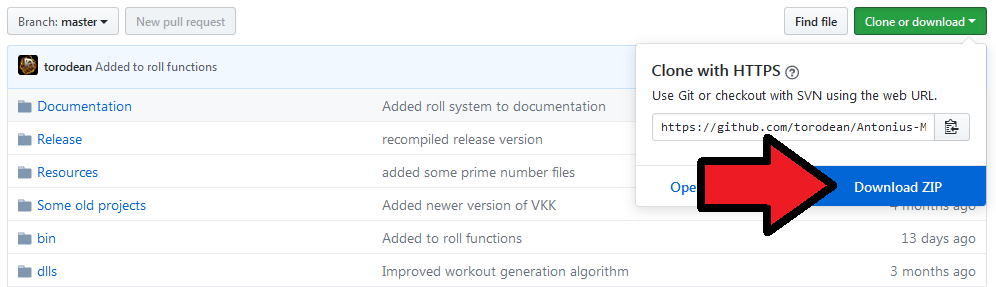
\includegraphics[width=0.9\textwidth]{images/setup01.png}
		\caption{The release folder.} \label{setup01}
	\end{figure}
	
	\item Select ``Save File" and then press ``OK" in the window that appears. All necessary MIA files will be downloaded here. Depending on your browser (i.e Firefox, Google Chrome, Internet Explorer, etc) the downloaded files will be placed somewhere (generally the downloads folder). See Fig. \ref{setup02} for this step.
	
	\begin{figure}[h]
		\centering
		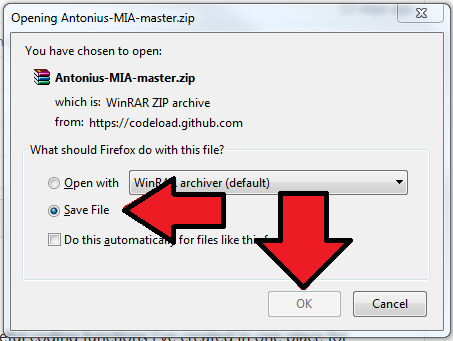
\includegraphics[width=0.4\textwidth]{images/setup02.png}
		\caption{The release folder.} \label{setup02}
	\end{figure}
	
	\item Navigate to your downloads folder. Right click on the ``Antonius-MIA-master.zip" that should have been downloaded. If you have WinRAR installed, select ``Extract here." If you have 7-ZIP installed, select ``7-ZIP", then ``Extract here." If you have another compression software installed, figure out how to extract it. If you do not have compression software installed you can do so easily by yourself or using Ninite (https://ninite.com/). See Fig. \ref{setup03} for this step.
	
	\begin{figure}[h]
		\centering
		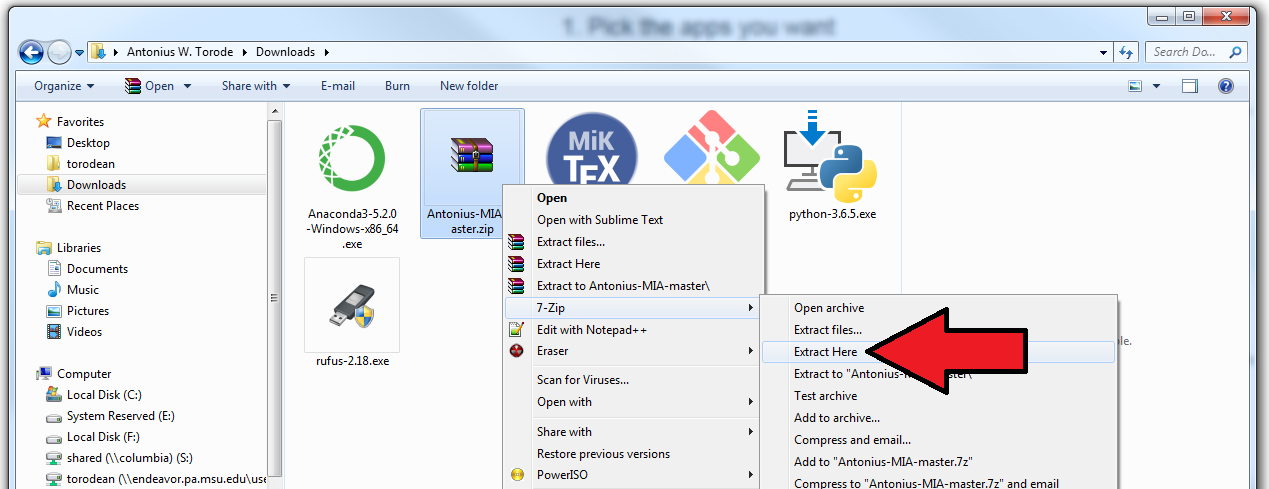
\includegraphics[width=0.9\textwidth]{images/setup03.png}
		\caption{The release folder.} \label{setup03}
	\end{figure}

	\item If done properly, a folder will have been created in your downloads folder called ``Antonius-MIA-master." You can move this folder to wherever you want the MIA program to be stored on your computer. Then, you can delete all items in the ``Antonius-MIA-master" folder EXCEPT the ``Release" folder, the ``README.md" file, and the ``Antonius’ General Purpose License (AGPL)" file. After doing so, you should be able to run and use MIA simple by opening the Release folder and clicking the ``MIA.exe" file as shown in figure \ref{setup04}.
	
	\begin{figure}[h]
		\centering
		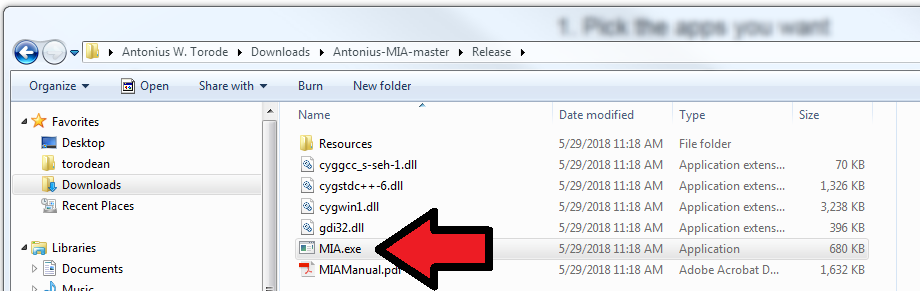
\includegraphics[width=0.9\textwidth]{images/setup04.png}
		\caption{The release folder.} \label{setup04}
	\end{figure}

\end{enumerate}